% -------------------- Packages --------------------

\documentclass{assignment}[2019/10/15]
\usepackage[lineno, pgfplots]{packages}[2019/10/15]
\pgfplotsset{compat=1.3}
\usetikzlibrary{arrows, backgrounds, positioning, fit}

% -------------------- Settings --------------------

% Title

\title{Homework of Chapter 5}
\author{Chen Xuyang}
\date{\today}
\institute{School of Mathematical Science}
\professor{Chen Xiongda}
\course{Operations Research}
\subject{Operations Research}
\keywords{}

% -------------------- New commands --------------------

\newcommand{\BR}{\symbb{R}}
\newcommand{\diag}{\mathop{}\!\symup{diag}}
\newcommand{\pr}{\mathop{}\!\symup{Pr}}
\newcommand{\expect}{\mathop{}\!\symup{E}}
\newcommand{\cov}{\mathop{}\!\symup{Cov}}
\newcommand{\var}{\mathop{}\!\symup{Var}}

% -------------------- Document --------------------

\begin{document}
    \maketitle
    \begin{problem}
        Implement Algorithm 5.2 (CG) and use it to solve linear systems in which $\matr{A}$ is the Hilbert matrix, whose elements are $\matr{A}_{i, j}=1/(i+j-1)$. Set the right-hand-side to $b=(1, 1, \dotsc, 1)^T$ and the initial point to $x_0=0$. Try dimensions $n = 5, 8, 12, 20$ and report the number of iterations required to reduce the residual below $10^{-6}$.
    \end{problem}
    \begin{solution}
        The result is listed in the following table and the codes are put into the appendix.
        \begin{table}[htb]
            \begin{center}
                \caption{The number of iterations required to reduce the residual below $10^{-6}$ of the linear systems as the dimension grows.}
                \pgfplotstabletypeset[
                    string type,
                ]{
                    {Dimension} {Number of Iterations}
                    5 6
                    8 19
                    12 51
                    20 279
                }
            \end{center}
        \end{table}
    \end{solution}
    \begin{problem}
        \begin{enumerate}[(a)]
            \item Show that if $f$ is strongly convex, then (6.7) holds for any vectors $x_k$ and $x_{k+1}$.
            \item Give an example of a function of one variable satisfying $g(0)=1$ and $g(1)=-1/4$ amd show that (6.7) does not hold in this case.
        \end{enumerate}
    \end{problem}
    \begin{proof}
        Without loss of generality, let's assume $f$ to be of one variable so that we can prove that each element of $s^Ty$ is positive.

        Since $f$ is strictly convex and differentiable, then $f'$ is strictly increasing. Hence there is the inequality
        \begin{equation}
            (x-y)(f'(x)-f'(y))>0
        \end{equation}
        for any distinct points $x$ and $y$. It follows the conclusion.

        An example is $g(x)=-4x^2/5+1$.
    \end{proof}
    \clearpage
    \begin{problem}
        Draw the adjacency graph for the function $f$ defined by (8.22). Show that the coloring scheme in which node $1$ has one color while nodes $2, 3, \dotsc, n$ have another color is valid. Draw the intersection graph for $\nabla f$.
    \end{problem}
    \begin{solution}
        The conclusion is naturally derived from the definition.
        \begin{figure}[htb]
            \centering
            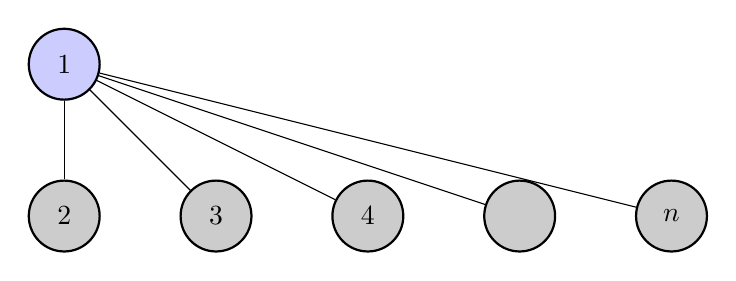
\begin{tikzpicture}
                [one/.style={circle, draw, fill=blue!20, thick, inner sep=0pt, minimum size=9mm},
                node/.style={circle, draw, fill=black!20, thick, inner sep=0pt, minimum size=9mm}]
                \node[one] (one) {1};
                \node[node] (two) [below=of one] {2};
                \node[node] (three) [right=of two] {3};
                \node[node] (four) [right=of three] {4};
                \node[node] (dots) [right=of four] {$\dotsc$};
                \node[node] (n) [right=of dots] {$n$};
                \draw [-] (one) to (two);
                \draw [-] (one) to (three);
                \draw [-] (one) to (four);
                \draw [-] (one) to (dots);
                \draw [-] (one) to (n);
            \end{tikzpicture}
            \caption{The adjacency graph for the function $f$ defined by (8.22)}
        \end{figure}
        \begin{figure}[htb]
            \centering
            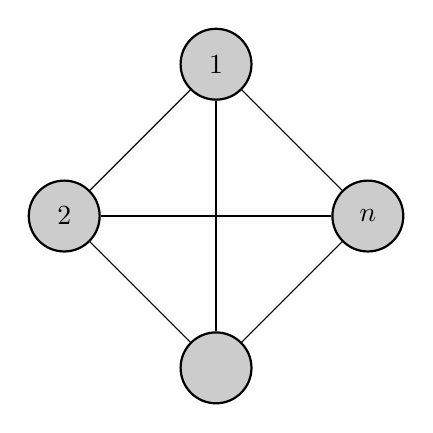
\begin{tikzpicture}
                [invisible/.style={circle, thick, inner sep=0pt, minimum size=9mm},
                node/.style={circle, draw, fill=black!20, thick, inner sep=0pt, minimum size=9mm}]
                \node[node] (one) {1};
                \node[invisible] (three) [below=of one] {};
                \node[node] (dots) [below=of three] {$\dotsc$};
                \node[node] (two) [left=of three] {2};
                \node[node] (n) [right=of three] {$n$};
                \draw [-] (one) to (two);
                \draw [-] (one) to (dots);
                \draw [-] (one) to (n);
                \draw [-] (two) to (dots);
                \draw [-] (two) to (n);
                \draw [-] (n) to (dots);
            \end{tikzpicture}
            \caption{The intersection graph for $\nabla f$}
        \end{figure}
    \end{solution}
    \begin{problem}
        Prove Lemma 9.1.
    \end{problem}
    \begin{problem}
        Prove that the generating set (9.24) satisfies the property (9.21) for a certain value $\delta>0$, and find this value of $\delta$.
    \end{problem}
    \begin{problem}
        Let $\matr{J}$ be an $m\times n$ matrix with $m\geq n$, and let $y\in\symbb{R}^m$ be a vector.
        \begin{enumerate}
            \item Show that $\matr{J}$ has full column rank if and only if $\matr{J}^T\matr{J}$ is nonsingular.
            \item Show that $\matr{J}$ has full column rank if and only if $\matr{J}^T\matr{J}$ is positive definite.
        \end{enumerate}
    \end{problem}
    \begin{proof}
        First, notice that linear equations $\matr{J}^T\matr{J}x=0$ and $\matr{J}x=0$ are equivalent, that is to say they have the same solutions. If $\matr{J}$ has full column rank, then the solution space has dimension $n$, which implies that $\matr{J}^T\matr{J}$ is nonsingular, and the converse is also true.

        Second, since $\matr{J}^T\matr{J}$ is always positive semi definite, $\matr{J}^T\matr{J}$ is nonsingular if and only if it is positive definite. It follows the conclusion.
    \end{proof}

    \clearpage\appendix
    \section{Codes}

    \matlabinputlisting[caption={Conjugate Gradient Method}]{conjugate_gradient.m}
\end{document}
